% !TEX root = main.tex
\documentclass[twocolumn]{article}
\usepackage[a4paper,margin=1in]{geometry} 
\usepackage{lmodern}
\usepackage{setspace}
\usepackage{mathptmx}
\usepackage{algorithm}
\usepackage{algpseudocode}
\usepackage{amsmath}
\usepackage{booktabs}
\usepackage{arydshln}
\usepackage{float}
\usepackage{cite}
\usepackage{multirow}
\usepackage{graphicx}
\usepackage{url}
\usepackage{import}
\usepackage{xcolor}

\title{\huge \textbf{Words That Matter:\\ Vocabulary Pruning in ModernBERT}}
\author{Wout De Rijck, Prof. Dr. Ir. Thomas Demeester, \\ Prof. Dr. Ir. Chris Develder, Karel D'Oosterlinck}
\date{} % No date

\begin{document}
\maketitle

\begin{abstract}

Large language models (LLMs) require substantial computational and memory resources, limiting their utility in resource-constrained environments. 
ModernBERT is a smaller encoder-only language model that excels at various tasks while being computationally highly efficient. 
In this work, we study how much more ModernBERT can be compressed while retaining accuracy on any given task.
Specifically, we introduce a series of very simple vocabulary pruning techniques that target the embedding layer. We compare the resulting accuracy with LoSparse, a state-of-the-art gradient-based pruning technique that targets the encoder layers.
For parameter reductions up to $\sim$20\%, our much simpler vocabulary pruning technique outperforms LoSparse, retaining on average 97.6\% of ModernBERT's performance across various tasks, compared to LoSparse's 92.9\%.
The strong performance of our simple technique indicates that task-specific pruning can meaningfully increase the efficiency of ModernBERT, an already highly efficient model. Additionally, our results suggest that state-of-the-art encoder-layer pruning can fall short of simple embedding-layer pruning.

\end{abstract}

\section{Introduction}
Language models need to be efficient for optimal deployment.
Efficiency can be assessed in several dimensions, including inference latency, throughput, energy consumption, parameter count, and memory usage.
In this work, we study how to optimally reduce the memory footprint of language models by removing unimportant vocabulary tokens from the embedding layer, resulting in faster model loading, reduced deployment costs, and improved accessibility for edge devices or resource-constrained environments.

\begin{figure}[t]
\centering
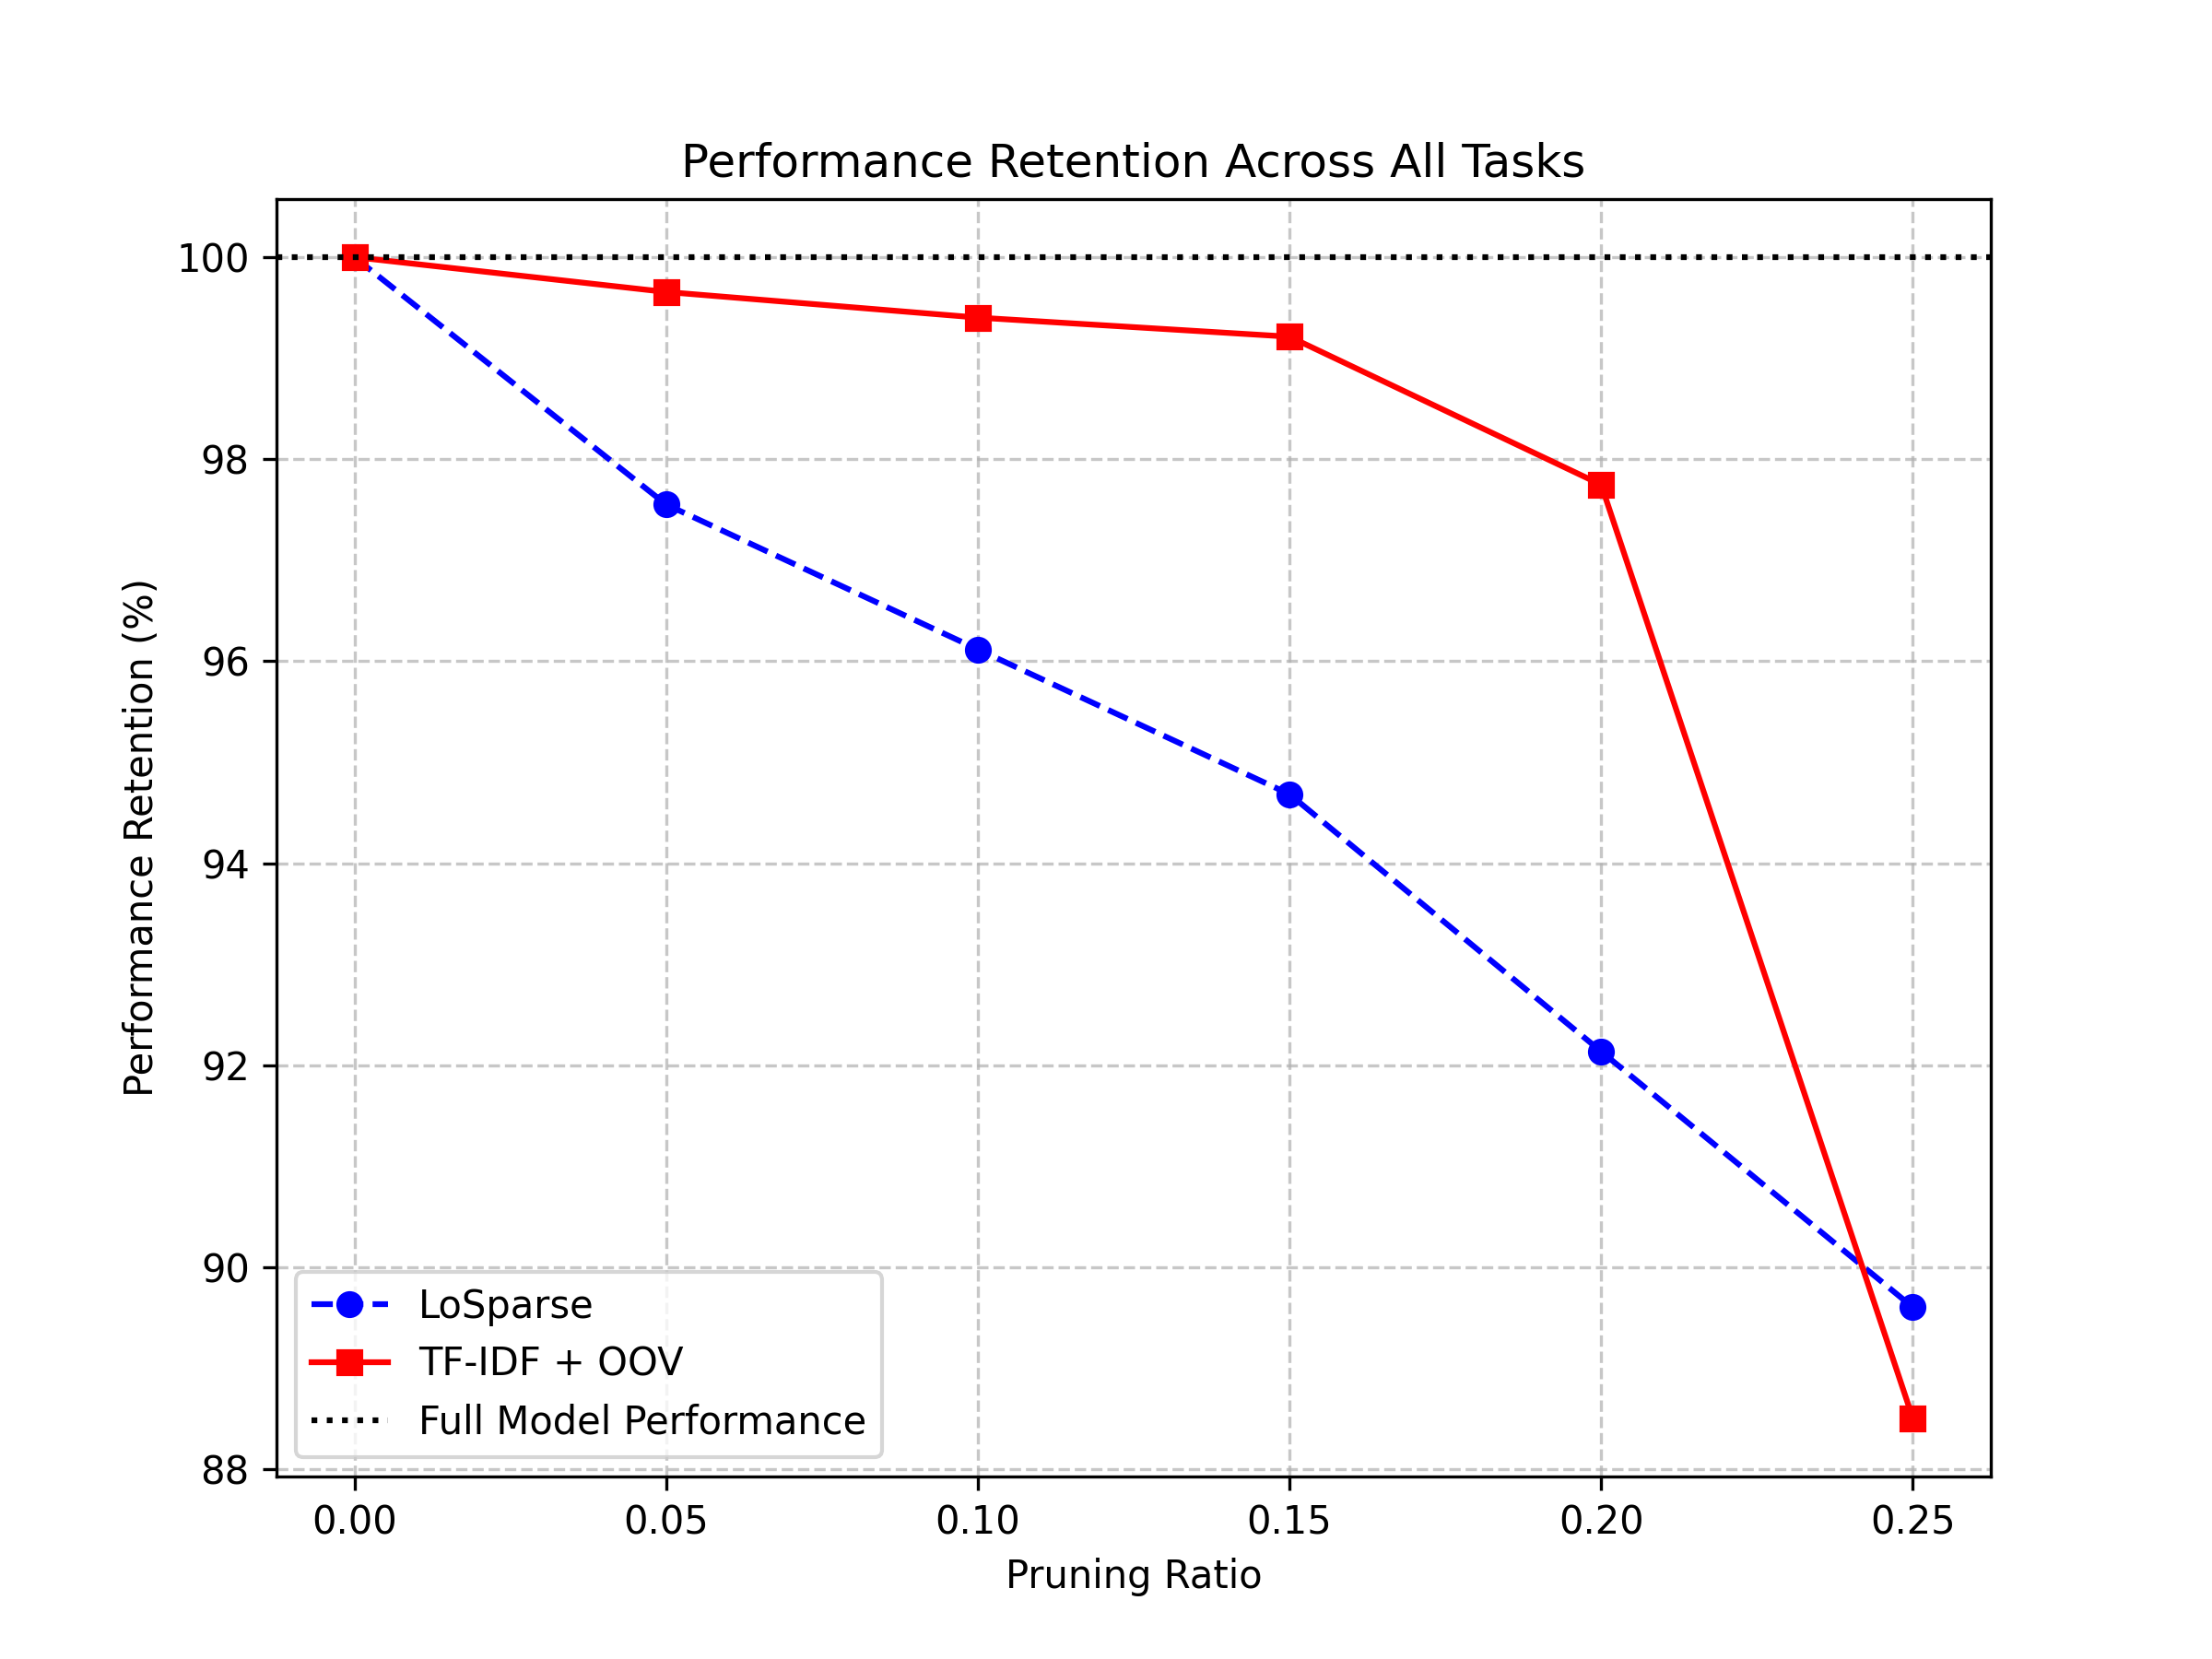
\includegraphics[width=\columnwidth]{images/performance_retention.png}
\caption{Average Performance Retention Across All Tasks for different pruning methods. Pruning ratio represents the fraction of total parameters removed from the model, limited to 0.25 as the embedding layer constitutes 25.95\% of all parameters.}
\label{fig:pruning_retention}
\end{figure}

From this perspective, ModernBERT stands out as one of the most lightweight and optimized encoder-only transformers available. It integrates several architectural and training innovations, successfully maintaining robust downstream performance while minimizing inference costs. Despite these advancements, a critical question remains open: Can we further enhance ModernBERT's efficiency by pruning parameters?

This question is particularly significant for two reasons. First, ModernBERT's inherent efficiency and its strong potential for large-scale deployment mean that optimal pruning strategies on top of this model could yield exceptionally efficient models. Second, existing research into pruning techniques have predominantly targeted decoder-only LLMs \cite{namburi2023llm} due to their widespread popularity, leaving encoder-only models relatively underexplored.

Specifically, we explore task-specific weight pruning, as ModernBERT is intended to be fine-tuned on specific tasks for optimal behavior (unlike more general-purpose decoder-only models that can utilize in-context learning). We hypothesize that simple task-specific pruning of the embedding matrix can be highly efficient, as many tokens can be irrelevant for any specific downstream task and the embedding layers counts for a significant portion ($\sim$25\% of the total parameters).

We explore a series of simple vocabulary pruning heuristics on a range of Natural Language Processing tasks including linguistic acceptability, sentiment analysis, paraphrase detection, semantic similarity, question answering, and natural language inference, as covered by the GLUE benchmark. For any task, we first apply this pruning to the base ModernBERT model and subsequently fine-tune the pruned model. For any given pruning ratio, we measure the accuracy retention compared to simply fine-tuning the model. We compare these vocabulary pruning techniques with LoSparse, a state-of-the-art gradient-based pruning technique that targets the encoder layers.

As shown in Figure \ref{fig:pruning_retention}, TF-IDF-based vocabulary pruning outperforms encoder-layer pruning (LoSparse) for compression ratios up to 20\%, maintaining 97.6\% of ModernBERT's original performance while removing 77.34\% of embedding parameters. This demonstrates that substantial efficiency gains can be achieved with virtually no performance loss using a simple, offline pruning technique. Beyond 20\% compression, performance drops sharply as we approach the embedding layer's parameter limit (25.95\% of total model parameters), while LoSparse maintains more stable performance at higher ratios. Unlike LoSparse, which requires computationally expensive gradient-based optimization, our vocabulary pruning operates as a straightforward pre-fine-tuning step with minimal overhead, making it particularly suitable for resource-constrained environments requiring moderate model compression.

\section{Related work}
Model compression techniques enhance the efficiency of large language models (LLMs) by reducing their size and computational requirements. Most modern LLM compression approaches operate under post-training settings, eliminating the need for resource-intensive retraining. Model compression strategies for LLMs can be categorized into four primary methods:

\begin{enumerate}
    \item Quantization: Reduces the numerical precision of model weights, decreasing memory footprint while maintaining reasonable performance.
    \item Parameter pruning: Eliminates redundant or less important connections and neurons to create sparser models with fewer parameters.
    \item Low-rank approximation: Decomposes weight matrices into lower-dimensional representations that capture essential information while requiring fewer parameters.
    \item Knowledge distillation: Transfers knowledge from larger teacher models to smaller student models, enabling competitive performance with reduced architecture size.
\end{enumerate}
These approaches are complementary and can be combined to achieve optimal compression from different perspectives. 
This work focuses on pruning techniques to reduce model size while preserving performance.
For ModernBERT, an encoder-only model, this research examines specific pruning methods for encoder layers and separate techniques for the embedding matrix.

\subsection{Encoder-Layer Pruning}

Encoder-layer pruning methods aim to remove redundant parameters within the transformer encoder to reduce model size while retaining accuracy. A representative example is \textbf{LoSparse}~\cite{li2023losparse}, which decomposes each weight matrix into a low-rank component and a sparse residual. The low-rank term captures the dominant shared subspace, while the sparse term accounts for residual variation. During fine-tuning, LoSparse uses first-order sensitivity scores—computed as the product of each weight and its gradient—to iteratively prune low-importance parameters. 

Several alternative encoder pruning techniques have been proposed. \textbf{Attention-head pruning}~\cite{michel2019sixteen} removes entire attention heads with minimal performance loss. \textbf{Movement pruning}~\cite{sanh2020movement} applies gradient-guided masking to gradually zero out low-importance weights during fine-tuning. \textbf{LayerDrop}~\cite{fan2020layerdrop} introduces structured dropout, allowing entire transformer layers to be stochastically removed during training and optionally pruned at inference.

These encoder-layer pruning methods differ in their granularity and strategy—targeting individual weights, attention heads, or full layers. Among them, LoSparse stands out as a strong baseline for encoder-level pruning.


\subsection{Embedding-Layer Compression}
Pruning the embedding layer often means removing or compressing rows (token vectors) to shrink this heavy component. \textbf{Partial Embedding Matrix Adaptation (PEMA)}~\cite{bousquet2023pema} temporarily removes unused tokens during fine-tuning and restores them afterward. It builds a partial embedding matrix containing only task-relevant tokens, reducing GPU memory requirements without compromising accuracy. 
Experiments show significant memory reductions: BERT$_{\text{BASE}}$'s embedding matrix shrinks by $\sim$47\%.
PEMA maintains full performance while making embedding pruning practical during training.

Another approach is \textbf{embedding compression} via factorization or hashing. \textbf{LightToken}~\cite{wang2023lighttoken} compresses the embedding matrix using low-rank SVD combined with a binary residual autoencoder. 
They note that token embeddings are highly redundant (comprising $\sim$21--31\% of BERT/RoBERTa's size). LightToken captures primary variations through rank-$k$ SVD, then uses compact hash codes for residuals. This achieves 25$\times$ smaller embeddings while maintaining accuracy—for BERT$_{\text{BASE}}$, it produces an average GLUE score of 82.9 versus the baseline 83.0.

These methods show that even structured low-rank or quantized pruning of embeddings can yield massive space savings with minimal impact on performance.

Overall, embedding-layer pruning techniques exploit the fact that many token vectors (especially for rare subwords) contribute little to end-task accuracy. By either dropping unused rows (PEMA/TextPruner) or factoring and quantizing embeddings (LightToken), these methods reduce $\sim$25--50\% of model parameters in the embedding matrix, enabling lighter models in practice.

\subsubsection{Vocabulary Pruning Techniques}
Vocabulary pruning removes rarely used or task-irrelevant tokens to shrink the model's vocabulary (and its embedding matrix). Early work by Abdaoui et al.~\cite{abdaoui2020load} showed that most parameters of multilingual BERT lie in the embedding layer, so trimming unused language tokens can dramatically cut size. In "Load What You Need," they drop languages from mBERT's vocabulary and obtain up to a 45\% reduction in total parameters with comparable accuracy on XNLI.

More recently, Nair et al.~\cite{nair2023blade} proposed \textbf{BLADE}, extending the implicit pruning in \textbf{SPLADE-X}~\cite{formal2023spladex} (which restricted output to query-language tokens). BLADE explicitly builds a pruned bilingual model containing only tokens from query and document languages, reducing parameters by $\sim$36.5\% versus full mBERT while speeding up training by $\sim$30\% and inference by $\sim$55\%, with minimal retrieval quality loss.

Dorkin et al.~\cite{dorkin2025estonian} also evaluated pruning for an Estonian adaptation: pruning all tokens unused by Estonian led to no degradation on NER, whereas retraining a new tokenizer hurt performance. These studies consistently find that deleting infrequently seen subwords yields large size savings with little accuracy drop.

\textbf{TextPruner} by Shen et al.~\cite{shen2022textpruner} uses a simple "drop unused tokens" technique: it scans a corpus and removes any tokenizer token not present in the text, deleting its row in the embedding matrix. This approach can cut model size and speed up training/inference on that domain.
\\ \\
Across tasks and languages, pruned-vocabulary models often match full models. For example, after pruning, Nair et al.~\cite{nair2023blade} report retrieval effectiveness on par with larger baselines, while achieving much faster indexing. Dorkin et al.~\cite{dorkin2025estonian} explicitly note "vocabulary pruning has no observable negative effect on the downstream task" (Estonian NER). These findings suggest vocabulary pruning is an effective way to tailor large models to specific domains or languages.

\newpage
\section{Method}
The proposed hybrid vocabulary pruning method for ModernBERT targets the embedding layer, which constitutes approximately 25\% of the model's parameters. This approach is based on the observation that tokens in a vocabulary have varying importance for downstream tasks, and that certain tokens can be selectively removed with minimal impact on performance. The method primarily consists of two main components: token importance analysis and selective pruning, with an optional third component: semantic clustering for out-of-vocabulary (OOV) tokens that can further enhance performance in some cases.

\subsection{Pre-Fine-Tuning Pruning Procedure}
In contrast to methods that require resource-intensive post-pruning fine-tuning, the proposed vocabulary pruning approach operates as a pre-fine-tuning offline optimization step in the model adaptation pipeline. The standard workflow for adapting ModernBERT to a downstream task involves taking the pre-trained base model and fine-tuning it directly on the task data. This research modifies this workflow as follows:

\begin{enumerate}
    \item Task data analysis: The downstream task dataset is processed to extract token statistics.
    \item Token importance calculation: Based on the analysis, tokens are ranked by their importance using one of several methods (frequency, TF-IDF, attention patterns, etc.).
    \item Vocabulary pruning: The embedding layer is pruned by removing less important tokens according to the calculated rankings.
    \item Optional OOV handling: For pruned tokens, semantic clustering may be applied to create mappings to representative tokens.
    \item Model fine-tuning: The pruned model is then fine-tuned on the downstream task using standard procedures.
\end{enumerate}
All pruning techniques follow these common steps:
\begin{enumerate}
    \item Always preserve special tokens ([CLS], [SEP], [PAD], etc.) regardless of their importance scores
    \item Calculate token importance using the technique-specific method
    \item Sort tokens by their importance scores in descending order
    \item Keep the top $(100-p)\%$ highest-scoring tokens, where $p$ is the pruning percentage
    \item Create a reduced embedding matrix using only the retained tokens
\end{enumerate}
This approach front-loads the pruning work to the pre-fine-tuning phase, meaning the actual fine-tuning process remains unchanged and operates on a model that already has a reduced parameter count. The resulting pruned model maintains its standard inference pipeline while benefiting from reduced memory requirements.

The high-level vocabulary pruning procedure, is formalized in Algorithm~\ref{alg:pre_ft_pruning}.

\begin{algorithm}[H]
\small
\caption{Pre-Fine-Tuning Vocabulary Pruning}
\label{alg:pre_ft_pruning}
\begin{algorithmic}[1]
\Require Pretrained model $M$ with vocab $V$, dataset $D$, pruning ratio $p$
\Ensure Pruned model $M'$
\State $\text{stats} \gets \text{compute\_token\_statistics}(D)$
\State $\text{scores} \gets \text{rank\_tokens}(\text{stats})$
\State $V_{\text{keep}} \gets \text{special\_tokens}(M)\cup\text{top\_k\_tokens}(\text{scores}, 1 - p)$
\State $M' \gets \text{rebuild\_model\_with\_vocab}(M, V_{\text{keep}})$
\State \Return $M'$
\end{algorithmic}
\end{algorithm}

\subsection{Token Importance Analysis}
A critical challenge in vocabulary pruning is determining which tokens to retain and which to remove. This research explores and compares several token importance estimation techniques, each with distinct theoretical foundations and practical implications for model performance. These approaches range from simple statistical methods to complex semantic analysis.

\subsubsection{Random Selection}
Tokens are pruned randomly without consideration for importance, serving as a baseline approach. In this method, tokens are selected for removal using uniform random sampling from the full vocabulary.

\subsubsection{Clustering-Based}
This approach employs agglomerative hierarchical clustering on the embedding space to group tokens with similar semantic properties. The algorithm works as follows:

\begin{enumerate}
    \item Each token's embedding vector is normalized to unit length (magnitude of 1), allowing the algorithm to compare tokens based solely on their semantic direction rather than magnitude.
    \item Agglomerative clustering begins with each token as its own cluster, then iteratively merges the closest pairs of clusters.
    \item The merging process uses average linkage, where the distance between clusters is the average distance between all pairs of embeddings across the two clusters.
    \item The algorithm stops when the target number of clusters is reached (determined by the pruning percentage).
    \item For each resulting cluster, the token closest to the centroid is identified and retained as the representative.
    \item All other tokens in the cluster are pruned from the vocabulary.
\end{enumerate}
This method preserves semantic diversity across the vocabulary while reducing redundancy. By selecting representatives closest to cluster centroids, the approach ensures that the preserved tokens maximize coverage of the semantic space. The clustering leverages the property that tokens with embeddings pointing in similar directions (high cosine similarity) tend to have similar semantic meanings, allowing one representative token to effectively substitute for multiple semantically related tokens.

\subsubsection{Frequency-Based}
Tokens are ranked by their frequency in the target dataset, with least frequently used tokens pruned first. This approach operates on the principle that rarely used tokens contribute less to model performance. The technique-specific algorithm steps are:

\begin{enumerate}
    \item Count occurrences of each token in the task-specific dataset
    \item Sort tokens by frequency (most common first)
\end{enumerate}
\subsubsection{Attention-Based}
This method leverages the attention mechanism of transformer models to identify important tokens. The key insight is that tokens receiving higher attention during inference are those the model relies on most heavily when making predictions, providing a direct measure of token importance from the model's perspective. Unlike frequency-based approaches that simply count occurrences, attention-based pruning preserves tokens that meaningfully contribute to the model's decision-making process.

For example, the important tokens identified in the SST-2 dataset differ markedly between methods. Frequency-based approaches naturally prioritize common words like articles and prepositions, while attention-based analysis highlights sentiment-laden terms that are semantically relevant to the classification task.
% \begin{figure*}[t]
% \centering
% \begin{minipage}{0.48\textwidth}
%   \centering
%   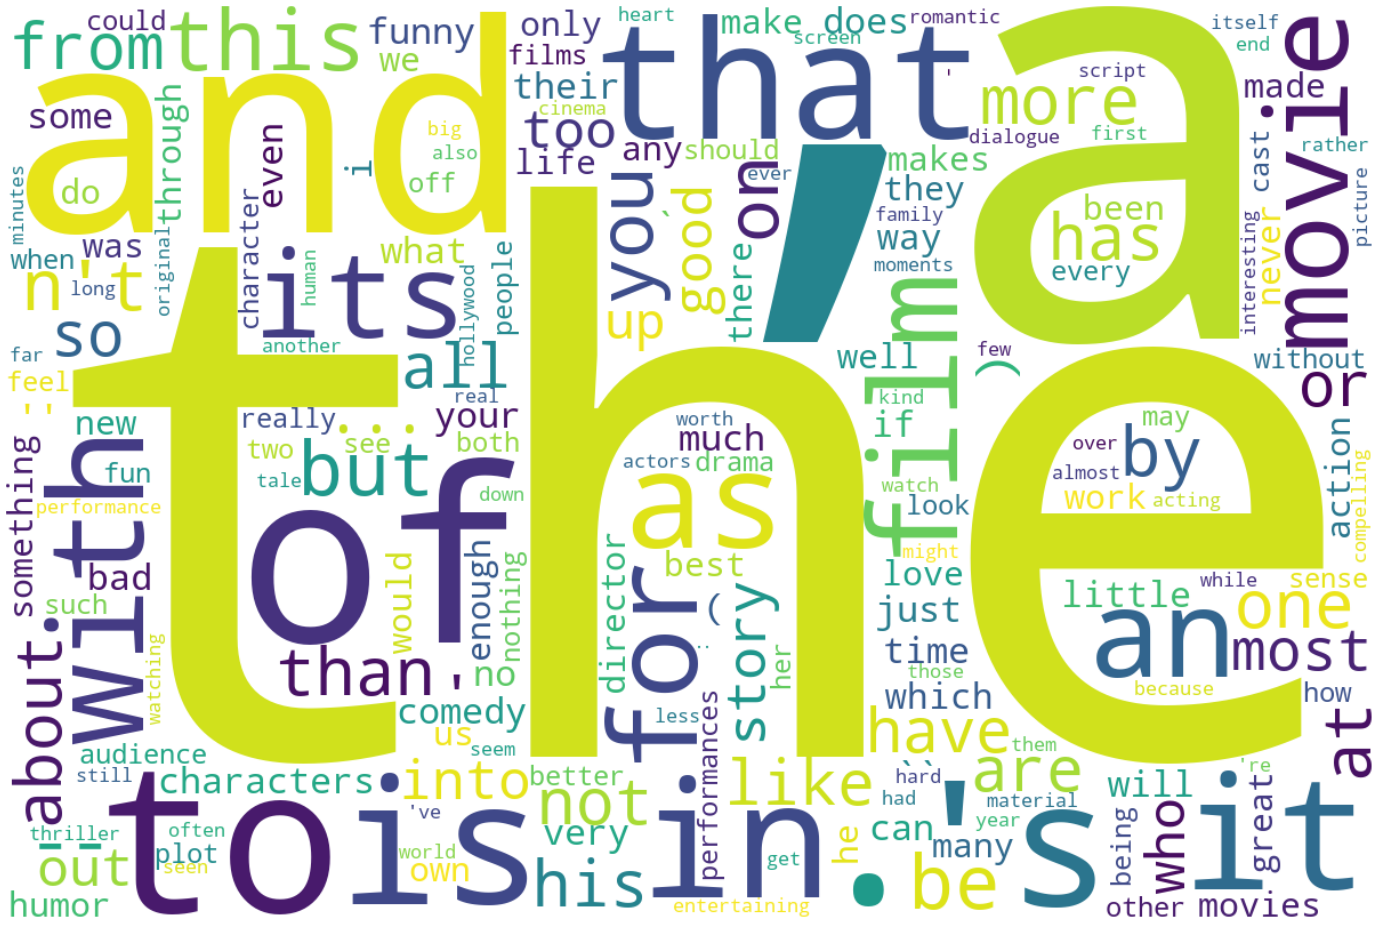
\includegraphics[width=\textwidth]{images/wordcloud_frequency.png}
% \end{minipage}%
% \hfill
% \begin{minipage}{0.48\textwidth}
%   \centering
%   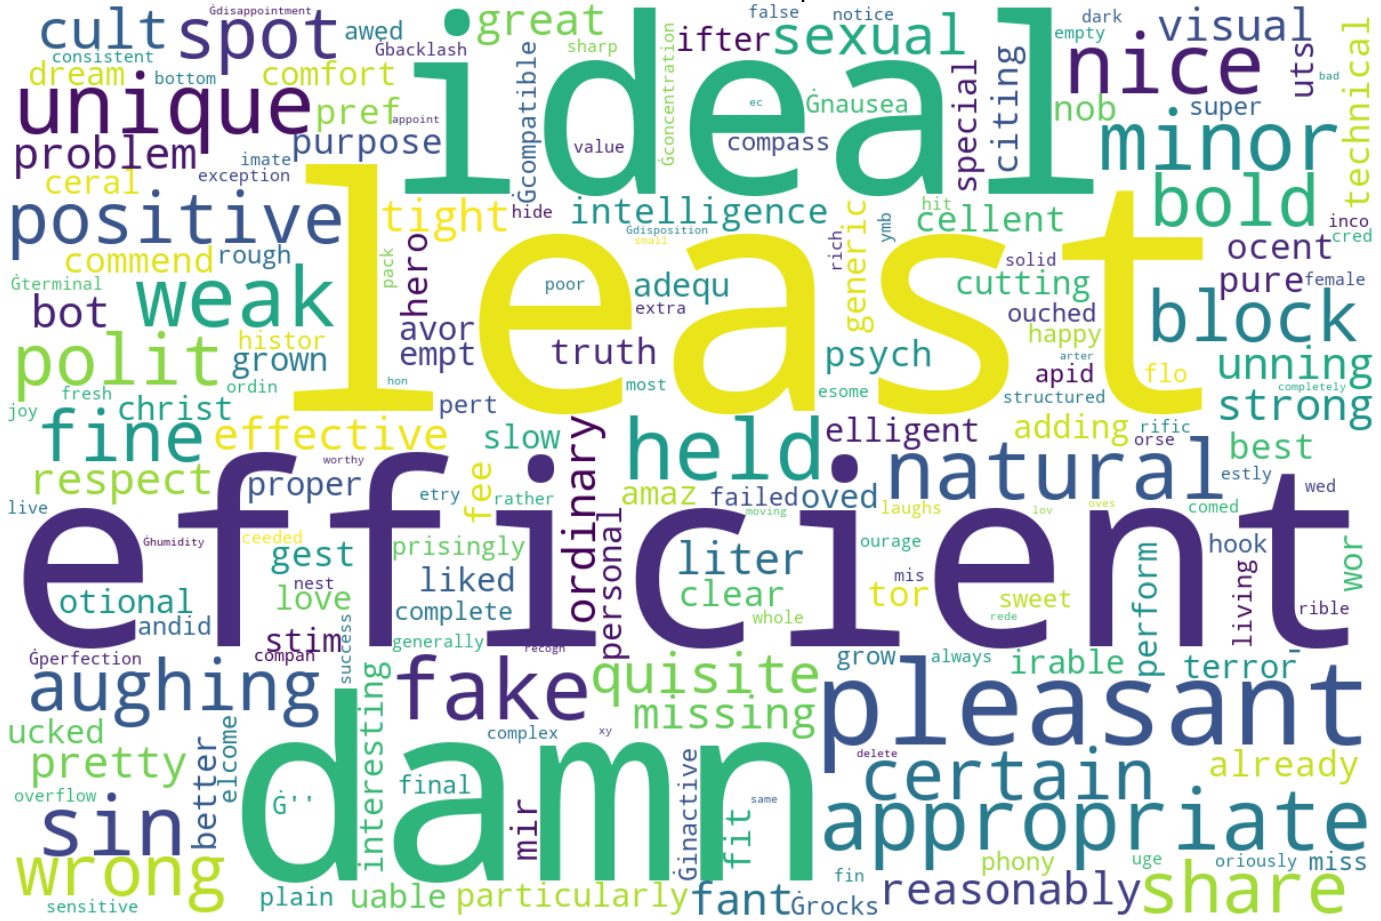
\includegraphics[width=\textwidth]{images/wordcloud_attention.png}
% \end{minipage}
% \caption{Comparison of top-ranked tokens for SST-2 task using frequency-based (left) versus attention-based (right) importance metrics.}
% \label{fig:wordcloud-comparison}
% \end{figure*}
% The visualization in Figure \ref{fig:wordcloud-comparison} demonstrates how attention-based pruning better captures task-relevant information, preserving tokens that carry greater semantic weight for the specific downstream task.
\\ \\
The technique-specific algorithm steps are:
\begin{enumerate}
    \item First fine-tune the base model on the target task to learn task-specific attention patterns
    \item Process the task dataset through this fine-tuned model, capturing attention matrices from all layers and heads
    \item For each token, aggregate the attention it receives across all contexts where it appears
    \item Normalize attention scores by token frequency to avoid bias toward common tokens
\end{enumerate}
\subsubsection{TF-IDF Based}
Tokens are ranked using Term Frequency-Inverse Document Frequency (TF-IDF) scores, which balance token occurrence frequency with discriminative power across documents. This method prioritizes tokens that appear frequently in specific documents but are rare across the corpus—capturing task-specific terminology while filtering out ubiquitous tokens that carry less semantic value.

The TF-IDF approach is particularly effective for tasks with distinct document categories (like sentiment classification or topic detection) where certain tokens strongly differentiate between classes. Unlike simple frequency counts, TF-IDF prevents common but semantically shallow tokens (articles, conjunctions, etc.) from dominating the pruned vocabulary.
\\ \\
The technique-specific algorithm steps are:
\begin{enumerate}
    \item Tokenize all examples in the task dataset
    \item Calculate term frequency (TF) for each token in each document:
        \begin{center}
        $\text{TF}(t,d) = \frac{\text{count of $t$ in $d$}}{\text{total terms in $d$}}$
        \end{center}
    \item Calculate inverse document frequency (IDF) across the corpus:
        \begin{center}
        $\text{IDF}(t) = \log\left(\frac{\text{total docs}}{\text{docs with $t$}}\right)$
        \end{center}
    \item Compute TF-IDF scores by multiplying TF and IDF values:
        \begin{center}
        $\text{TF-IDF}(t,d) = \text{TF}(t,d) \times \text{IDF}(t)$
        \end{center}
    \item Apply normalization to the scores (see variants below)
\end{enumerate}
For this approach, three normalization variants were implemented and evaluated:
\begin{itemize}
    \item Non-normalized TF-IDF: Raw scores that heavily prioritize rare but task-specific tokens
    \item L1-normalized TF-IDF: Scores normalized by sum, balancing frequency and discriminative power
    \item L2-normalized TF-IDF: Scores normalized by Euclidean norm, the standard approach in information retrieval that prevents outlier tokens from dominating
\end{itemize}
\subsection{Out-of-Vocabulary Token Handling}
The handling of out-of-vocabulary (OOV) tokens presents an opportunity to preserve additional semantic information during vocabulary pruning. While standard approaches typically map all pruned tokens to a single UNK token, this approach utilizes the semantic properties of the embedding space to maintain some of the original meaning of pruned tokens. This can help mitigate performance degradation by retaining partial semantic value for tokens not included in the reduced vocabulary.
\\ \\
The clustering-based OOV handling process works as follows:
\begin{enumerate}
    \item Extract embeddings for all tokens marked for removal during pruning
    \item Apply K-means clustering to these embeddings, grouping semantically similar tokens together
    \item For each cluster, identify the token closest to the centroid as the representative
    \item Create a mapping from each pruned token to its cluster representative
    \item During inference, when an OOV token is encountered, it is dynamically mapped to its assigned representative rather than the generic UNK token
\end{enumerate}
This approach maintains semantic nuance by ensuring that pruned tokens are replaced by semantically similar alternatives rather than a single catchall token. For example, domain-specific terminology might be mapped to more common synonyms, or rare morphological variants might be mapped to their common forms (e.g., "stabilized" → "stable"). The method is particularly effective for technical vocabularies where semantically related terms form natural clusters in the embedding space.

The number of clusters (k) provides a tunable parameter to balance compression rate against semantic precision—larger values of k preserve more semantic distinctiveness but reduce the overall pruning benefit. 
% TODO: Add experimental results and a plot
%Experimental results show that even a modest number of clusters (50-100) significantly improves model performance compared to a single UNK mapping approach.


\begin{table}[htbp]
\centering
\scriptsize
\setlength{\tabcolsep}{3pt}
\begin{tabular}{l|cc|cc|cc|c}
\toprule
\textbf{Task} & \multicolumn{2}{c|}{\textbf{Unique Tokens}} & \multicolumn{2}{c|}{\textbf{Vocab Cov. (\%)}} & \multicolumn{2}{c|}{\textbf{Top 20\%}} & \textbf{OOV} \\
 & \textbf{Train} & \textbf{Test} & \textbf{Train} & \textbf{Test} & \textbf{Train} & \textbf{Test} & \textbf{\%} \\
\midrule
COLA & 5,416 & 1,934 & 17.74 & 6.34 & 85.12 & 74.68 & 8.74 \\
MNLI & 25,793 & 22,664 & 84.51 & 74.25 & 90.69 & 89.64 & 0.14 \\
MRPC & 11,096 & 3,567 & 36.35 & 11.69 & 83.17 & 71.80 & 13.04 \\
QNLI & 26,176 & 20,360 & 85.76 & 66.71 & 88.31 & 85.79 & 0.41 \\
QQP & 25,486 & 18,534 & 83.50 & 60.72 & 94.02 & 91.79 & 1.03 \\
RTE & 13,354 & 4,198 & 43.75 & 13.75 & 81.77 & 70.75 & 12.12 \\
SST2 & 11,536 & 8,084 & 37.80 & 26.49 & 84.23 & 80.53 & 0.42 \\
STSB & 10,346 & 3,271 & 33.90 & 10.72 & 82.66 & 71.30 & 13.70 \\
\bottomrule
\end{tabular}
\caption{Token statistics across GLUE tasks, comparing train and test splits. OOV\%: percentage of test vocabulary not found in train.}
\label{tab:token_statistics}
\end{table}

\section{Experiments}
After developing several algorithmic approaches to vocabulary pruning, this section presents a comprehensive evaluation designed to answer several key questions: Can selective vocabulary reduction maintain model performance while significantly decreasing parameter count? How do different pruning strategies compare on various natural language understanding tasks? Does the pre-fine-tuning approach that avoids post-pruning recovery fine-tuning deliver practical benefits in real-world deployment scenarios? Through careful experimentation across diverse tasks, the results demonstrate not only the effectiveness of these algorithms but also their practical advantages in creating more efficient transformer models.

\subsection{Datasets and Metrics}
The General Language Understanding Evaluation (GLUE) benchmark serves as the primary evaluation framework for this study. GLUE consists of eight diverse natural language understanding tasks categorized into three groups: single-sentence tasks (SST-2, CoLA), similarity and paraphrase tasks (MRPC, STS-B, QQP), and natural language inference tasks (MNLI, QNLI, RTE). Performance metrics vary by task: classification tasks report accuracy; CoLA reports Matthew's correlation coefficient, and STS-B reports Pearson correlation.

Table \ref{tab:token_statistics} presents a detailed analysis of token distributions across all GLUE tasks. This analysis reveals significant vocabulary redundancy, with the top 20\% of tokens covering 80-94\% of all token occurrences in training sets. This finding provides strong empirical justification for vocabulary pruning, as most tokens contribute minimally to overall corpus coverage. The table also quantifies the overlap between TF-IDF and frequency-based token selection, showing substantial differences (38-60\% overlap), which explains the performance variations between these approaches.

Table \ref{tab:vocab_overlap} examines train-test vocabulary overlap, quantifying the percentage of out-of-vocabulary (OOV) tokens in test sets. While datasets like MNLI and QNLI show excellent coverage (less than 0.5\% OOV tokens), others such as MRPC, STSB, and RTE exhibit higher OOV percentages (12-14\%), highlighting the importance of effective OOV handling strategies in the pruning process. 

\begin{table}[htbp]
\centering
\scriptsize
\setlength{\tabcolsep}{4pt}
\begin{tabular}{l|cc}
\toprule
& \multicolumn{2}{c}{\textbf{Test Vocabulary Coverage}} \\
\textbf{Task} & \textbf{OOV Tokens} & \textbf{OOV\%} \\
\midrule
SST2 & 34 & 0.42\% \\
MRPC & 465 & 13.04\% \\
COLA & 169 & 8.74\% \\
STSB & 448 & 13.70\% \\
QQP & 191 & 1.03\% \\
MNLI & 31 & 0.14\% \\
QNLI & 83 & 0.41\% \\
RTE & 509 & 12.12\% \\
\bottomrule
\end{tabular}
\caption{Train-test vocabulary overlap statistics. \textbf{OOV Tokens}: number of unique tokens in the test set that don't appear in the training set; \textbf{OOV\%}: percentage of test vocabulary not found in train. Lower percentages indicate better vocabulary coverage, which is beneficial for pruning.}
\label{tab:vocab_overlap}
\end{table} 

\begin{table*}[h]
\centering
\scriptsize
\setlength{\tabcolsep}{9pt}
\begin{tabular}{l@{\hspace{25pt}}ccccccccc}
\toprule
& \multicolumn{2}{c}{\textbf{Single Sentence}} & \multicolumn{3}{c}{\textbf{Paraphrase and Similarity}} & \multicolumn{3}{c}{\textbf{Natural Language Inference}} & \multirow{2}{*}{\makebox[-20pt][c]{\vrule width 0.5pt height 175pt}\hspace{35pt}} \\
\cmidrule(lr){2-3} \cmidrule(lr){4-6} \cmidrule(lr){7-9}
\textbf{Method} & \textbf{SST-2} & \textbf{CoLA} & \textbf{MRPC} & \textbf{STS-B} & \textbf{QQP} & \textbf{MNLI} & \textbf{QNLI} & \textbf{RTE} & \textbf{AVG} \\
\midrule
\multicolumn{10}{l}{\textbf{Baseline}} \\
ModernBERT (Full) & 0.951 & 0.632 & 0.89 & 0.917 & 0.917 & 0.881 & 0.939 & 0.643 & 0.846 \\
\midrule
\multicolumn{10}{l}{\textbf{Vocabulary Pruning}} \\
Train Tokens Only & 0.950 & 0.630 & 0.861 & 0.917 & 0.917 & 0.883 & 0.915 & 0.639 & 0.839 \\
\textit{Parameter Reduction} & \textit{18.85\%} & \textit{22.61\%} & \textit{18.56\%} & \textit{18.76\%} & \textit{4.79\%} & \textit{6.74\%} & \textit{6.42\%} & \textit{17.06\%} & \textit{14.22\%} \\
\\ [-6pt]
\hdashline
\\[-6pt]
Random Selection & 0.911 & 0.470 & 0.798 & 0.845 & 0.780 & 0.504 & 0.669 & 0.566 & 0.693 \\
Clustering-Based & 0.894 & 0.188 & 0.752 & 0.696 & 0.871 & 0.683 & 0.833 & 0.566 & 0.685 \\
Attention-Based & \textbf{0.947} & 0.589 & \textbf{0.864} & 0.885 & 0.763 & 0.683 & 0.791 & 0.578 & 0.763 \\
Simple Frequency-Based & 0.943 & 0.467 & 0.812 & 0.905 & 0.904 & 0.858 & 0.902 & 0.546 & 0.792 \\
TF-IDF Based & 0.933 & 0.520 & 0.807 & 0.901 & 0.898 & 0.860 & 0.909 & 0.610 & 0.805 \\
\\ [-6pt]
\hdashline
\\[-6pt]
Simple Frequency + OOV & 0.938 & 0.540 & 0.828 & \textbf{0.906} & \textbf{0.915} & 0.858 & 0.907 & 0.615 & 0.813 \\
TF-IDF + OOV & 0.934 & \textbf{0.615} & 0.834 & 0.903 & 0.912 & 0.858 & \textbf{0.910} & \textbf{0.635} & \textbf{0.825} \\
\textit{Parameter Reduction} & \textit{20.25\%} & \textit{23.27\%} & \textit{20.02\%} & \textit{20.18\%} & \textit{20.02\%} & \textit{20.02\%} & \textit{20.02\%} & \textit{20.02\%} & \textit{20.48\%} \\
\midrule
\multicolumn{10}{l}{\textbf{Encoder Layer Pruning}} \\
LoSparse & 0.935 & 0.525 & 0.856 & 0.887 & \textbf{0.915} & \textbf{0.871} & 0.906 & 0.614 & 0.814 \\
\textit{Parameter Reduction} & \textit{20.16\%} & \textit{20.16\%} & \textit{20.16\%} & \textit{20.16\%} & \textit{20.16\%} & \textit{20.16\%} & \textit{20.16\%} & \textit{20.16\%} & \textit{20.16\%} \\
\bottomrule
\end{tabular}
\caption{Performance on GLUE dev set. ModernBERT is fine-tuned separately for each task. Scores are accuracies except for CoLA (Matthew's correlation), and STS-B (Pearson correlation). Notation "+ OOV" indicates pruning with out-of-vocabulary clustering. At 20\% parameter reduction, TF-IDF + OOV maintains 97.6\% of the original performance and outperforms LoSparse (0.825 vs 0.810 average score). OOV handling improves results by 2.0 percentage points on average.}

\label{tab:results}
\end{table*}

\subsection{Baselines}
Three baseline models are established to evaluate the effectiveness of the proposed vocabulary pruning techniques:

\begin{itemize}
    \item \textbf{ModernBERT (Full)}: The original pre-trained model with no modifications, representing the upper bound of performance with full parameter count. This baseline utilizes the complete 50,368-token vocabulary and all encoder parameters.
    \item \textbf{LoSparse}: An encoder-layer pruning technique that applies structured sparsification to reduce parameters in the self-attention and feed-forward networks. The implementation uses a low-rank plus sparse factorization that preserves 80\% of the original parameters across all encoder layers while keeping the embedding layer intact. This baseline represents a complementary approach that targets different model components.
    \item \textbf{Train Tokens Only}: A vocabulary reduction approach that removes all token embeddings not observed in the fine-tuning dataset. This method represents an upper bound for vocabulary pruning performance, as it preserves all task-relevant tokens without further reduction. All subsequent pruning techniques begin with this training vocabulary and apply additional selection criteria. The parameter reduction varies significantly by task (4.79-22.61\%), depending on vocabulary coverage in each dataset.
\end{itemize}
These baselines establish comparative benchmarks for assessing both the parameter efficiency and performance of the proposed vocabulary pruning methods. The full model provides the performance ceiling, LoSparse demonstrates the impact of encoder-only pruning, and the Train Tokens Only approach represents the simplest form of vocabulary reduction without sophisticated token selection criteria.

\subsection{Implementation Details}
All experiments were conducted on an NVIDIA RTX 4090 GPU. The vocabulary pruning techniques described in this paper were implemented in a public repository\footnote{\url{https://github.com/WoutDeRijck/vocab-pruning.git}}. This implementation includes all pruning methods, evaluation scripts, and analysis tools described in this work. For encoder layer pruning, a custom fork of the LoSparse implementation was used\footnote{\url{https://github.com/WoutDeRijck/LoSparse.git}}. Both codebases are released to facilitate reproducibility and further research in model compression techniques.

\begin{figure*}[t]
    \centering
    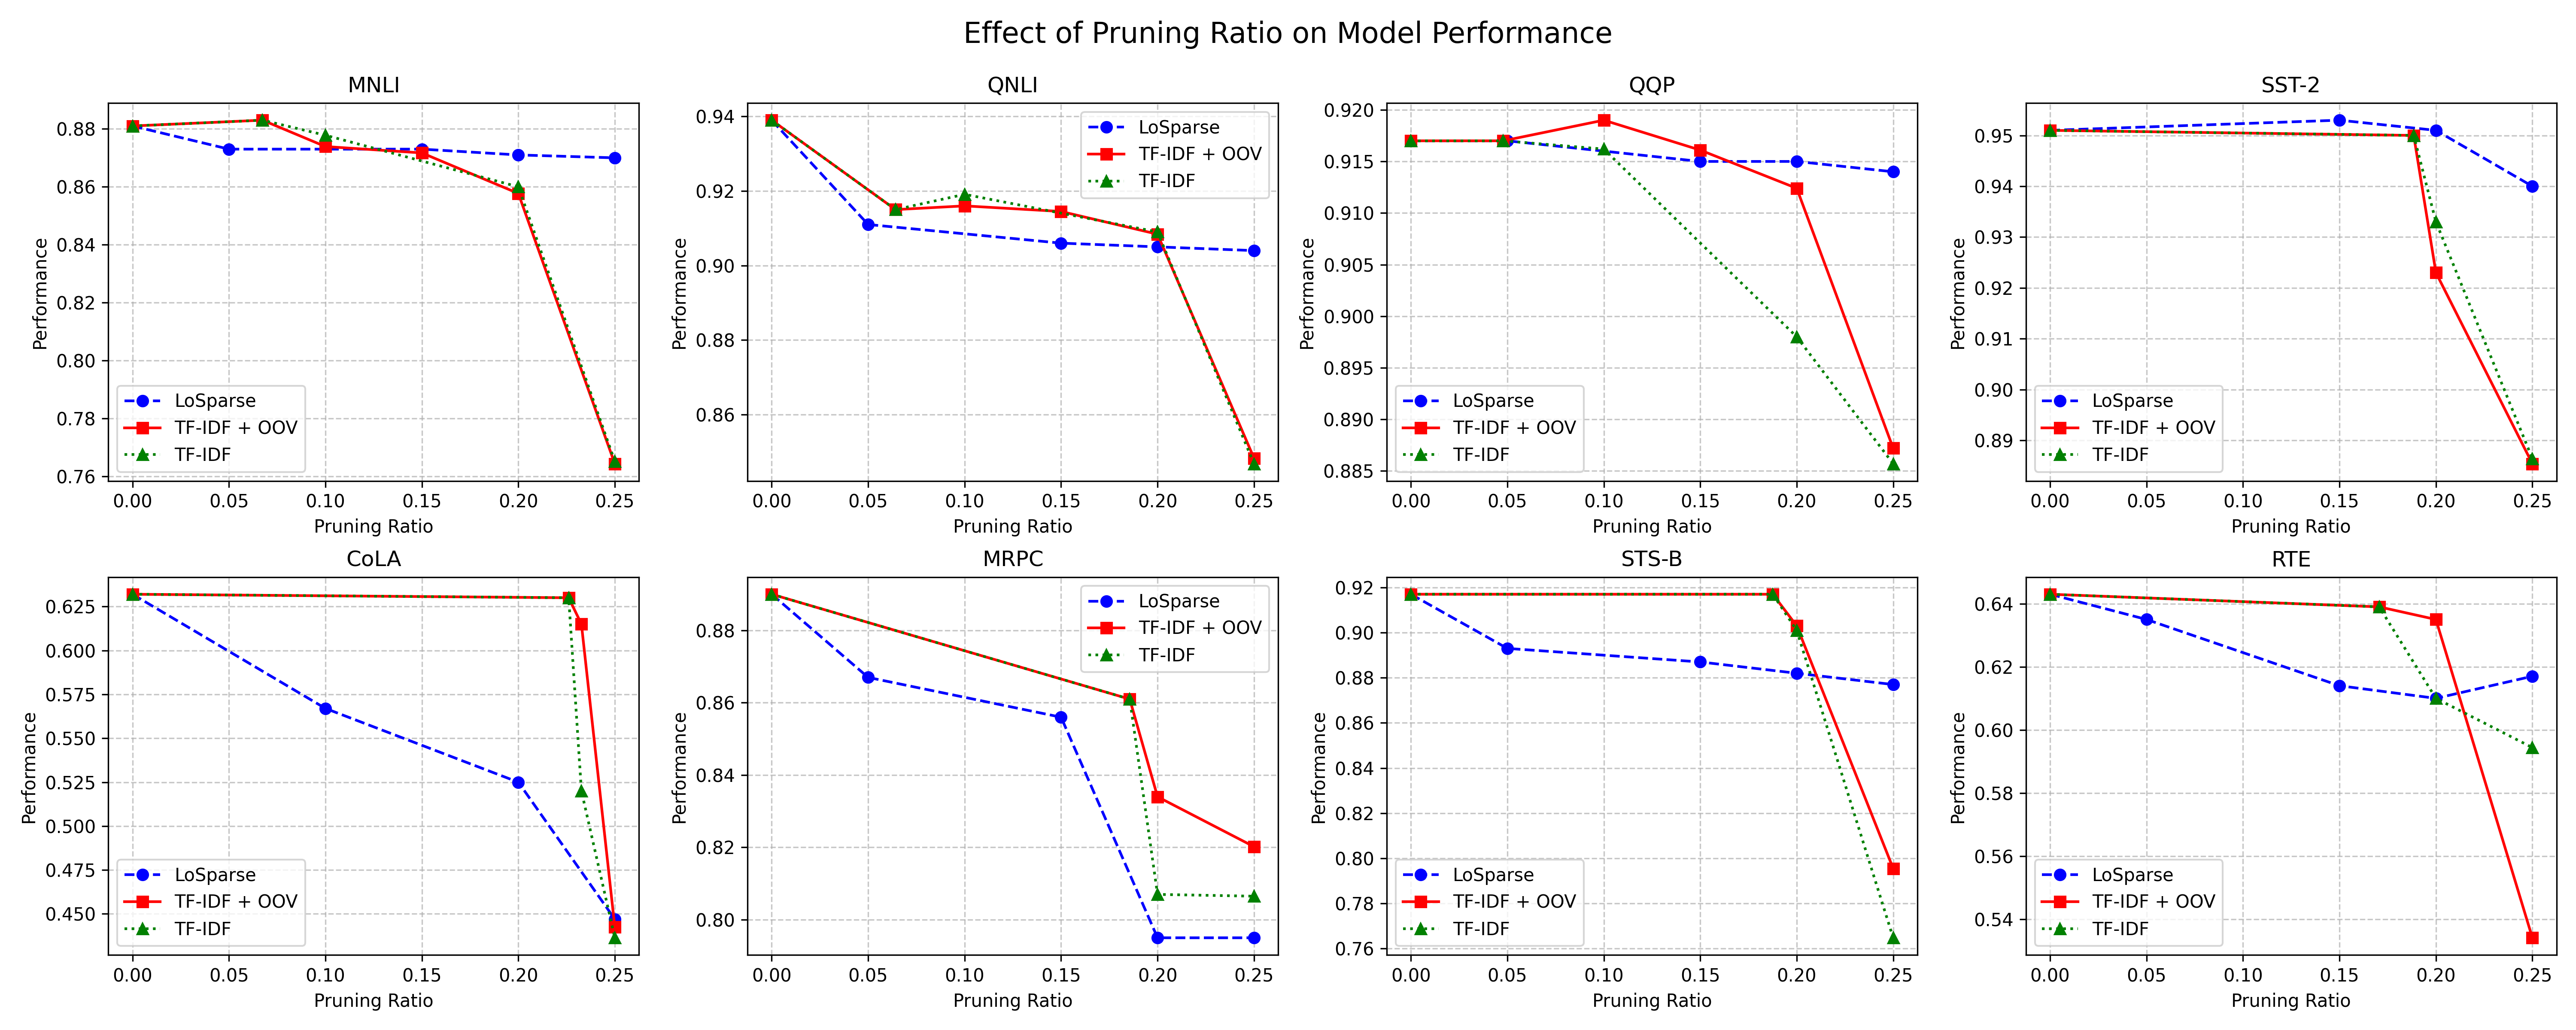
\includegraphics[width=\linewidth]{images/pruning_ratios.png}
    \caption{Performance comparison between vocabulary pruning (TF-IDF + OOV) and encoder pruning (LoSparse) across different pruning ratios for MNLI, QNLI, and QQP tasks. }
    \label{fig:pruning_ratio}
\end{figure*}

\subsection{Results}
Table \ref{tab:results} presents the comprehensive evaluation across all GLUE tasks for the different pruning methods. Several key findings emerge.

First, vocabulary pruning alone achieves substantial parameter reduction (20.02-23.27\%) with minimal performance impact. The TF-IDF + OOV approach performs exceptionally well, maintaining 97.6\% of the original model's average performance while reducing parameters by over 20\%.

Second, the inclusion of OOV handling mechanisms significantly improves results compared to their non-OOV counterparts. For instance, TF-IDF + OOV outperforms standard TF-IDF by 2.4 percentage points on average, with particularly strong improvements on CoLA (9.5 points) and RTE (6.1 points).

Third, the effectiveness of pruning varies across tasks. Attention-based pruning excels on single-sentence tasks (SST-2, CoLA) and paraphrase detection (MRPC), while TF-IDF-based methods perform better on more complex reasoning tasks (MNLI, QNLI, RTE).

Fourth, as illustrated in Figure \ref{fig:pruning_ratio}, vocabulary pruning demonstrates superior performance and efficiency compared to encoder-layer pruning (LoSparse) at lower pruning ratios (5-20\%). Importantly, while LoSparse requires computationally expensive online training procedures, vocabulary pruning is an offline pre-fine-tuning method that can be applied with minimal computational overhead. A striking result is that a 20\% reduction in total model parameters translates to a 77.34\% reduction in vocabulary size while maintaining competitive performance. This efficiency advantage makes vocabulary pruning particularly attractive for resource-constrained environments. Since the embedding layer constitutes only 25.95\% of the total model parameters, vocabulary pruning has an inherent upper limit. Beyond the 20\% threshold, performance decreases sharply for vocabulary pruning while LoSparse maintains more stable performance at higher compression rates. Vocabulary pruning provides an optimal approach for applications requiring moderate compression with minimal performance impact, while more aggressive compression could benefit from combining both techniques.

The benchmark results in Table \ref{tab:benchmark_results} further quantify the practical benefits, showing a 20\% reduction in storage size and 14.83\% reduction in GPU memory requirements with negligible impact on inference time (+1.33\%).

\begin{table}[htb]
\centering
\scriptsize
\setlength{\tabcolsep}{3pt}
\begin{tabular}{lrrr}
\toprule
\textbf{Metric} & \textbf{Base} & \textbf{Pruned} & \textbf{Impr.(\%)} \\
\midrule
Params (M) & 149.61 & 119.69 & 20.00 \\
Embed. Params (M) & 38.68 & 8.76 & 77.34 \\
Storage (MB) & 570.72 & 456.59 & 20.00 \\
GPU Mem (MB) & 823.06 & 700.99 & 14.83 \\
Infer. Time (ms) & 18.73 & 18.98 & -1.33 \\
\bottomrule
\end{tabular}
% \caption{Benchmark results comparing base ModernBERT with pruned variant.}
% \caption{Benchmark results comparing base ModernBERT with pruned variant during inference on an RTX 4090.}
\caption{Benchmark results comparing base ModernBERT with pruned variant (TF-IDF + OOV) during inference on an RTX 4090. Our method achieves 20\% reduction in total parameters (77.34\% of embedding parameters) and a 14.83\% reduction in GPU memory with negligible impact on inference time.}

\label{tab:benchmark_results}
\end{table} 


\section{Conclusion}

% This paper introduced a novel vocabulary pruning approach for transformer-based language models that eliminates the need for post-pruning recovery fine-tuning while delivering substantial parameter reduction with minimal performance impact. The work highlights the embedding layer as a critical yet often overlooked component for model compression, demonstrating that intelligent token selection can maintain 97.6\% of original model performance while reducing total parameters by 20-23\%.

% The key contributions of this research are:

% \begin{itemize}
%     \item A vocabulary pruning methodology that operates as a pre-fine-tuning optimization step, eliminating the need for post-pruning recovery fine-tuning typically associated with model compression.
    
%     \item A systematic comparison of token importance estimation techniques, revealing that TF-IDF with OOV handling provides the most robust performance across diverse NLP tasks.
    
%     \item Empirical evidence that vocabulary pruning outperforms encoder-based pruning at lower pruning ratios (5-20\%), offering a more efficient pathway for moderate model compression.
    
%     \item Practical deployment benefits including 20\% reduction in storage size and 14.83\% reduction in GPU memory with no inference time penalty.
% \end{itemize}

% The results challenge the conventional wisdom that encoder-layer pruning should be prioritized over vocabulary reduction. Instead, the findings demonstrate that a hybrid approach—focusing first on vocabulary pruning for initial efficiency gains and then applying encoder pruning for more aggressive compression—offers the most balanced pathway to efficient transformer models.

% The broader implications of this work extend beyond the specific techniques presented. By eliminating the need for expensive post-pruning fine-tuning, the presented approach democratizes model compression, making it accessible even for organizations with limited computational resources. This could accelerate the adoption of transformer models in resource-constrained environments such as mobile devices, edge computing platforms, and regions with limited technological infrastructure.

% Future work could explore dynamic vocabulary pruning that adapts to changing data distributions, application of these techniques to multilingual models where vocabulary redundancy is even more pronounced, and integration with quantization and knowledge distillation for more comprehensive compression pipelines. As large language models continue to grow in size and capability, efficient adaptation methods like vocabulary pruning will become increasingly critical for bridging the gap between research advances and practical deployment.

\section{Future Work}
TODO (these are just things I thought about)

\begin{itemize}
    \item \textbf{Unified Compression Framework}: Developing an integrated approach that combines vocabulary pruning with encoder-layer compression techniques like LoSparse could provide a more comprehensive model compression solution. Preliminary experiments suggest these approaches are complementary, with vocabulary pruning excelling at lower compression ratios and encoder pruning maintaining better performance at higher ratios.
    
    \item \textbf{Task Adaptation Networks}: Instead of removing pruned token embeddings entirely, future work could explore low-dimensional adapter networks that efficiently transform a small set of base embeddings to approximate the full vocabulary, potentially offering better performance/size tradeoffs.
    
    \item \textbf{Retrieval Performance Analysis}: Evaluating vocabulary pruning on information retrieval tasks could reveal different optimal pruning strategies, as retrieval models may depend on different token importance distributions than classification tasks.

\end{itemize}
\newpage
\bibliographystyle{plain}
\bibliography{references}

\end{document}
